\documentclass[journal,10pt]{IEEEtran}

\usepackage{cite}
\usepackage{amsmath,amssymb,amsfonts}
\usepackage{algorithmic}
\usepackage{graphicx}
\usepackage{textcomp}
\usepackage{xcolor}
\usepackage{booktabs}
\usepackage{multirow}
\usepackage{tikz}
\usetikzlibrary{arrows.meta,positioning,shapes.geometric,fit,backgrounds,calc}
% Coloured links (blue) without boxes
\usepackage[colorlinks=true, linkcolor=blue, citecolor=blue, urlcolor=blue]{hyperref}
\usepackage{balance}

% No need for \usepackage{url} – hyperref already handles it

\def\BibTeX{{\rm B\kern-.05em{\sc i\kern-.025em b}\kern-.08em
    T\kern-.1667em\lower.7ex\hbox{E}\kern-.125emX}}

\begin{document}
\title{Query-Efficient Adaptive Model Extraction of Vision Foundation Models:\\
A Pilot-Scale Empirical Study of Attack Strategy, Stealth, and Defense Trade-offs}

\author{
Raja Siraj Gul,
Sir Zaigham Abdullah Bin Qasim,
Zohha Bint E Sajjad, 
and Kolawole John Adebayo 
\thanks{
Raja Siraj Gul and Sir Zaigham Abdullah Bin Qasim are with the School of Computing Sciences, Pak-Austria Fachhochschule Institute of Applied Sciences and Technology, Haripur, Khyber Pakhtunkhwa, Pakistan (e-mail: rajasiraj755@gmail.com; sirzaighamabq@gmail.com).
}
\thanks{
Zohha Bint E Sajjad is with the Department of IT \& AI, University of Haripur, Haripur, Khyber Pakhtunkhwa, Pakistan(e-mail: zohha981@gmail.com).
}
\thanks{
Kolawole John Adebayo is with Maynooth University, Maynooth, Co. Kildare, Ireland (e-mail: kolawole.adebayo@mu.ie).
}
\thanks{Corresponding author: Kolawole John Adebayo.}
}

\markboth{IEEE Transactions on Information Forensics and Security, Vol.~XX, No.~X, Month 2026}
{}

\maketitle

\begin{abstract}
Model-extraction (model-stealing) attacks let an adversary clone the functionality of a deployed
machine-learning model by querying its prediction application programming interface (API) and
training a surrogate on the observed input--output pairs, without any access to the victim's
architecture, parameters, or training data. As vision foundation models such as vision transformers
(ViTs) and contrastive language--image pre-training (CLIP) encoders are increasingly deployed behind
pay-per-query interfaces, the query efficiency of the attacker's sampling strategy becomes the
central lever governing both the cost of an attack and the cost of defending against it. This paper
studies an adaptive query-selection strategy, $S(x)=\alpha\,U(x)+\beta\,D(x)+\gamma\,I(x)$, that
linearly combines surrogate-predictive uncertainty $U(x)$, embedding-space diversity $D(x)$, and an
information-gain proxy $I(x)$ to prioritise which unlabelled candidate images are sent to the
victim's application programming interface. We benchmark the adaptive strategy against random,
class-balanced, uncertainty-only, and diversity-only baselines, and against two published few-call
and data-free extraction baselines, across convolutional neural network (CNN), ViT, and
CLIP victim families on CIFAR-10 and an ImageNet-derived subset. We further instrument three
attacker stealth levels (naive, rate-mimicking, stealth-optimized) and a behavioural
extraction-risk detector, and quantify the resulting security--utility trade-off under a graduated,
risk-scored defense across three defense-strength settings. Using five-seed statistics with
95\% confidence intervals, we find that the adaptive strategy does not uniformly dominate a random
baseline at the query budgets tested on CIFAR-10 ($t=-3.35$, $p=0.029$, Cohen's $d=-1.50$, favouring
random), while showing a markedly larger fidelity gain at the larger, more realistic ImageNet-derived
scale, and that CLIP-style victims are consistently the most vulnerable of the three families tested.
A six-feature behavioural detector nearly doubles recall against a stealth-optimized attacker
relative to a four-feature baseline (0.56 vs.\ 0.22) at zero false-positive rate on the sessions
tested. We report these results as a pilot-scale, compute-constrained study and explicitly scope
the claims accordingly, situating them within 27 papers on model extraction attacks and defenses
published between 2021 and 2025.
\end{abstract}

\begin{IEEEkeywords}
model extraction, active learning, black-box attacks, vision-language models, extraction detection
\end{IEEEkeywords}


\section{Introduction}
\label{sec:intro}

Machine-learning-as-a-service (MLaaS) platforms expose trained models through prediction
application programming interfaces (APIs) that return a label, a top-$k$ ranking, or a full
confidence vector for each submitted query. This convenience creates a well-documented attack
surface: an adversary with no knowledge of the victim's architecture, parameters, or training
distribution can repeatedly query the API, collect the returned soft or hard labels, and use them
to train a local \emph{surrogate} (or \emph{student}) model that approximates the victim's
decision function. Such \emph{model extraction} (or \emph{model stealing}) attacks compromise the
intellectual property embedded in a deployed model, can act as a stepping stone toward
transferable adversarial examples, and increasingly target not only classical convolutional
networks but also vision foundation models -- vision transformers (ViTs) and contrastive
vision--language encoders like CLIP -- that are expensive to train and are precisely the assets
an MLaaS provider most wants to protect~\cite{dosovitskiy2021vit,radford2021clip}.

Because each query typically has a monetary or rate-limit cost, the central practical question for
an attacker is \emph{which} unlabelled candidate inputs to query, and for a defender it is how to
detect and disrupt that query pattern without degrading service for legitimate users. Early attacks
queried public data at random~\cite{orekondy2019knockoff-context} or used active-learning-style
uncertainty sampling~\cite{pal2020activethief-context}; more recent work has explored data-free
and few-call regimes that synthesise proxy queries instead of relying on a public dataset at
all~\cite{truong2021dfme,kariyappa2021maze,sanyal2022hardlabel,hondru2025aspkd,zhuang2025stealix},
and a parallel literature has developed defenses ranging from prediction perturbation and
watermarking to behavioural detection of extraction
sessions~\cite{jia2021entangled,szyller2021dawn,tang2024modelguard,zhou2024inversionguided}.
Despite this volume of work, three gaps remain salient for vision \emph{foundation} models
specifically. First, most query-selection strategies were designed and evaluated against
convolutional victims; how they transfer to ViT and CLIP-style victims is comparatively
under-studied. Second, few studies combine an adaptive query strategy with an explicit,
multi-level attacker stealth model and a matched behavioural defense, so the security--utility
trade-off curve as a function of defense strength is rarely reported. Third, few-call/data-free
baselines and active-query baselines are rarely benchmarked against each other under an identical
protocol.

This paper reports a pilot-scale empirical study that addresses these three gaps under an explicit,
declared compute budget (a single-GPU, free-tier setting), rather than at the full architectural
and data scale of a well-resourced attacker. Concretely, we:

\begin{itemize}
\item formalise and implement an adaptive query-selection strategy
$S(x)=\alpha\,U(x)+\beta\,D(x)+\gamma\,I(x)$ that combines predictive uncertainty, embedding-space
diversity, and a perturbation-sensitivity proxy for information gain, and compare it against
random, class-balanced, uncertainty-only, and diversity-only baselines, and against two published
few-call/data-free baselines (ASPKD~\cite{hondru2025aspkd} and a simplified Stealix-style
prompt-evolution baseline~\cite{zhuang2025stealix});
\item evaluate all strategies against three victim families -- a ResNet-style CNN, a small ViT, and
a CLIP ViT-B/32 image encoder with a linear probe -- on CIFAR-10, and validate the strongest
configuration on an ImageNet-derived (Imagenette) subset;
\item instrument three attacker stealth levels (naive, rate-mimicking, stealth-optimized) and train
a behavioural extraction-risk detector, comparing a four-feature and a six-feature variant;
\item couple the detector to a graduated, risk-scored defense and trace the resulting
security--utility trade-off curve across three defense-strength settings; and
\item report five-seed statistics with 95\% confidence intervals for the core strategy comparison
and explicitly scope our claims to the tested architectures, budgets, and dataset scale.
\end{itemize}

We emphasise at the outset that this is a \emph{pilot-scale} study, constrained to a single
free-tier graphics processing unit (GPU) with a weekly quota. The core comparisons use a
ResNet-18 convolutional surrogate on CIFAR-10 with five random seeds; the ViT, CLIP, and
Imagenette-scale results use one seed per configuration. We report this scope explicitly rather
than implicitly generalising pilot-scale point estimates to claims about full-scale foundation-model
deployments, consistent with recommended practice for compute-constrained systems-security
studies~\cite{oliynyk2023survey,zhao2025systematic}.

\subsection{Organization}

The remainder of this paper is organised as follows. Section~\ref{sec:related} reviews the
literature on model extraction attacks and defenses published in the past five years.
Section~\ref{sec:threat} states the threat model. Section~\ref{sec:method} describes the
methodology, including the victim models, the query API, the candidate pool, the baseline and
adaptive query strategies, the attack loop, the stealth levels, and the detector/defense pipeline.
Section~\ref{sec:setup} describes the experimental setup. Section~\ref{sec:results} reports
results. Section~\ref{sec:discussion} discusses limitations and threats to validity.
Section~\ref{sec:conclusion} concludes.

\section{Related Work}
\label{sec:related}

We organise the past five years (2021--2025) of model-extraction literature into four themes:
(A) query-efficient and active-learning-based attacks; (B) data-free and few-call attacks that
avoid a public query dataset entirely; (C) attacks and defenses specific to self-supervised
encoders and vision--language models, the family most relevant to CLIP-style victims; and
(D) defenses, watermarking, and behavioural detection of extraction sessions. We close with recent
surveys that synthesise this space.

\subsection{Query-Efficient and Active-Learning-Based Extraction}

A central line of work treats query selection as an active-learning problem: the attacker
maintains a partially trained surrogate and prioritises candidate queries that are maximally
informative under that surrogate, rather than sampling uniformly. Battis and Penner
extend this idea specifically to transformer-based victims, showing that extraction strategies
tuned for convolutional networks transfer imperfectly to ViT-style targets and that
architecture-aware query selection narrows the gap~\cite{battis2022vitextraction}. Karmakar and
Basu formalise \emph{distributional equivalence} rather than pointwise agreement as the attacker's
objective and propose Marich, a query-efficient strategy that explicitly targets matching the
victim's output distribution under a fixed query budget~\cite{karmakar2023marich}. Jindal et
al.\ show that an ensemble of diverse candidate-selection heuristics, combined via a
sample-selection ensemble, out-performs any single heuristic (uncertainty, diversity, or
class-balance alone) at a fixed budget, which is consistent with the multi-term composition of the
adaptive strategy studied in this paper~\cite{jindal2024armyofthieves}. Chen et al.\ study the
attacker's side of the arms race directly, proposing a defense-penetrating extraction framework
(D-DAE) that detects when victim outputs have been perturbed by a disruption-based defense and
adaptively recovers an unperturbed estimate before selecting the next query batch, which
motivates our own inclusion of an adaptive, risk-scored defense rather than a static
one~\cite{chen2023ddae}.

\subsection{Data-Free and Few-Call Extraction}

A second line of work removes the assumption that the attacker has access to an unlabelled public
dataset that resembles the victim's training distribution. Truong et al.\ and Kariyappa et al.\
independently introduced data-free model extraction, using a generator trained adversarially (or
via zeroth-order gradient estimation through the victim) to synthesise query images directly,
removing the public-dataset assumption at the cost of a substantially larger query
budget~\cite{truong2021dfme,kariyappa2021maze}. Sanyal et al.\ extend data-free extraction to the
hard-label setting, where only the arg-max class -- not a confidence vector -- is
observable~\cite{sanyal2022hardlabel}, which is directly relevant to MLaaS deployments that
return only a predicted label. Hondru and Ionescu propose Active Self-Paced Knowledge
Distillation (ASPKD), which generates a large proxy dataset with a diffusion model, queries only a
small, actively selected subset of it against the victim, pseudo-labels the remainder via
latent-space nearest-neighbour propagation from the surrogate, and trains with a self-paced
curriculum that introduces harder pseudo-labelled samples only once the surrogate is
confident~\cite{hondru2025aspkd}; this is one of the two published few-call baselines we
reproduce. Zhuang et al.\ remove the need for a hand-crafted text prompt or known class names
entirely, using a genetic prompt-evolution procedure over a pre-trained diffusion model to infer
the victim's data distribution from its own responses, and show this out-performs
manually-prompted diffusion-based baselines including ASPKD under a matched query
budget~\cite{zhuang2025stealix}; we reproduce a simplified version of this Stealix-style baseline.

\subsection{Encoder- and Vision-Language-Model Extraction}

Because our victim families include a CLIP-style linear-probe encoder, we highlight the literature
specific to self-supervised and contrastive encoders. Liu et al.\ show that pre-trained encoders
can be stolen with an $L_2$-based imitation loss on returned embedding vectors alone, without any
downstream labels, establishing that encoder-level theft is both feasible and cheaper than
attacking each downstream classifier separately~\cite{liu2022stolenencoder}. Sha et al.\ propose
Cont-Steal, which shows that a \emph{contrastive} imitation loss -- rather than simple
embedding-distance regression -- is a substantially more effective attack against encoders trained
with contrastive objectives, which is the training regime underlying CLIP-style
victims~\cite{sha2023contsteal}. On the defensive side, Dziedzic et al.\ formally study why
self-supervised encoders are \emph{harder} to defend than supervised classifiers, because a
defender cannot easily perturb a high-dimensional embedding without destroying its
utility~\cite{dziedzic2022ssldefense}, and follow up with Bucks-for-Buckets (B4B), an active
defense that perturbs returned embeddings in proportion to an estimate of how much of the
embedding space a given client has already covered, directly motivating the diversity-aware
component of adaptive query strategies as something a defender can also track and
penalise~\cite{dziedzic2023b4b}.

\subsection{Defenses, Watermarking, and Behavioural Detection}

A large body of defensive work perturbs or otherwise degrades the victim's returned predictions.
Jia et al.\ propose entangled watermarks, which force the victim's decision boundary to entangle
a small set of watermark samples with the legitimate task such that a surrogate trained on stolen
queries inherits the watermark behaviour and can later be used for ownership
verification~\cite{jia2021entangled}. Szyller et al.\ propose DAWN, a dynamic watermarking scheme
that perturbs a small fraction of \emph{responses} (rather than training-time behaviour) in a
way that is detectable in a suspect model without harming task
accuracy~\cite{szyller2021dawn}. Tang et al.\ and Tan et al.\ each propose watermark designs
explicitly evaluated for robustness against extraction, rather than only against fine-tuning or
pruning, using transferable trigger sets and multi-view training data
respectively~\cite{tang2023exposingtheft,tan2023dnnwatermark}, and Zhu et al.\ study the
robustness--evasion trade-off directly, showing that watermarks tuned purely for extraction
robustness are more easily detected and stripped by an adaptive
attacker~\cite{zhu2024reliablewatermark}. Beyond watermarking, Tang et al.\ propose ModelGuard, an
information-theoretic prediction-perturbation defense derived from an explicit optimisation
problem over the attacker's achievable fidelity, and show it dominates prior heuristic
perturbation defenses against \emph{adaptive} attackers that attempt to detect and undo
perturbation~\cite{tang2024modelguard}. Zhou et al.\ take a detection-first approach, using an
auxiliary inversion model to flag sessions whose query distribution is inconsistent with normal
usage~\cite{zhou2024inversionguided}, which is conceptually the same behavioural-detection
strategy we implement, and Nayan et al.\ provide a systematisation of knowledge for on-device
extraction that emphasises the persistent gap between what defenses are evaluated in research and
what is deployed in practice~\cite{nayan2024sok}. Zhao et al.\ report a superpixel-based
gradient attack that improves query efficiency for extraction under a fixed
budget~\cite{zhao2024superpixel}, illustrating that the attacker side of this arms race continues
to advance alongside the defenses above.

\subsection{Surveys}

Three recent surveys synthesise this space and are complementary to the present study. Oliynyk et
al.\ provide the first broad taxonomy spanning attacks, defenses, and their evaluation
methodology up to 2023~\cite{oliynyk2023survey}. Zhao et al.\ provide a 2025 systematic survey
that updates this taxonomy with foundation-model and large-language-model extraction, and note
explicitly that architecture-aware and stealth-aware evaluation -- the two axes emphasised in this
paper -- remain comparatively under-studied relative to attack novelty
alone~\cite{zhao2025systematic}. A companion survey by the same group focuses specifically on
extraction of large language models and defenses against
it~\cite{zhao2025llmsurvey}, which we do not evaluate directly but note as the natural extension
of the vision-model threat model studied here to the text modality.

\begin{table*}[t]
\centering
\caption{Summary of the 27 Reviewed Papers (2021--2025), Grouped by Theme}
\label{tab:litreview}
\begin{tabular}{@{}p{0.150\textwidth}p{0.280\textwidth}p{0.150\textwidth}p{0.055\textwidth}p{0.225\textwidth}@{}}
\toprule
\textbf{Theme} & \textbf{Representative works} & \textbf{Victim type} & \textbf{Year} & \textbf{Core idea} \\
\midrule
Active/query-efficient attacks &
Battis \& Penner~\cite{battis2022vitextraction}; Karmakar \& Basu~\cite{karmakar2023marich};
Jindal et al.~\cite{jindal2024armyofthieves}; Chen et al.~\cite{chen2023ddae} &
CNN, ViT & 2022--24 & Prioritise informative / diverse / defense-penetrating queries \\
\addlinespace
Data-free / few-call attacks &
Truong et al.~\cite{truong2021dfme}; Kariyappa et al.~\cite{kariyappa2021maze};
Sanyal et al.~\cite{sanyal2022hardlabel}; Hondru \& Ionescu~\cite{hondru2025aspkd};
Zhuang et al.~\cite{zhuang2025stealix} &
CNN & 2021--25 & Synthesise queries; no public data or hand-crafted prompts required \\
\addlinespace
Encoder / VLM extraction \&\ defense &
Liu et al.~\cite{liu2022stolenencoder}; Sha et al.~\cite{sha2023contsteal};
Dziedzic et al.~\cite{dziedzic2022ssldefense,dziedzic2023b4b} &
Self-supervised / contrastive encoder & 2022--23 & Steal / defend embedding-level representations (relevant to CLIP) \\
\addlinespace
Defenses, watermarking, detection &
Jia et al.~\cite{jia2021entangled}; Szyller et al.~\cite{szyller2021dawn};
Tang et al.~\cite{tang2023exposingtheft,tang2024modelguard}; Tan et al.~\cite{tan2023dnnwatermark};
Zhu et al.~\cite{zhu2024reliablewatermark}; Zhou et al.~\cite{zhou2024inversionguided};
Nayan et al.~\cite{nayan2024sok}; Zhao et al.~\cite{zhao2024superpixel} &
CNN, general & 2021--24 & Watermark, perturb, or behaviourally detect extraction sessions \\
\addlinespace
Surveys / background &
Oliynyk et al.~\cite{oliynyk2023survey}; Zhao et al.~\cite{zhao2025systematic,zhao2025llmsurvey};
Dosovitskiy et al.~\cite{dosovitskiy2021vit}; Radford et al.~\cite{radford2021clip} &
-- & 2021--25 & Taxonomy, and the ViT/CLIP architectures used as victims here \\
\bottomrule
\end{tabular}
\end{table*}

\subsection{Positioning of This Work}

Table~\ref{tab:litreview} summarises the reviewed literature. Relative to this body of work, the
present study does not propose a fundamentally new attack primitive; instead, it (i) evaluates an
adaptive, multi-term query-selection strategy against \emph{three} victim families spanning CNN,
ViT, and CLIP -- whereas most cited attacks are evaluated on a single convolutional victim family
-- (ii) benchmarks that active-query strategy directly against two published data-free/few-call
baselines under a matched query budget, which the active-learning and data-free literatures
rarely do against each other, and (iii) couples an explicit three-level attacker stealth model to
a graduated, risk-scored defense and reports the resulting security--utility trade-off \emph{curve}
across defense strengths, rather than a single operating point, extending the single-point
evaluations typical of the watermarking and detection literature reviewed above.

\section{Threat Model}
\label{sec:threat}

We adopt a standard black-box extraction threat model. The victim $V$ is a trained classifier
deployed behind a query interface that accepts an image $x$ and returns either a hard label, a
top-$k$ ranking, or a full confidence vector, depending on the configured \emph{output-knowledge}
variant. The attacker $A$ has (i) no access to $V$'s architecture, parameters, or training data;
(ii) access to a \emph{public candidate pool} of unlabelled images, disjoint from $V$'s private
training split; (iii) a fixed query budget $B$; and (iv) the ability to incrementally fine-tune a
local surrogate model $\hat V$ after each queried batch. The attacker's goal is to maximise
\emph{fidelity} -- agreement between $\hat V$ and $V$ on a held-out evaluation set -- within the
budget $B$. We additionally model three attacker \emph{stealth} levels that vary how the query
stream is paced and spatially distributed in embedding space, and a defender that can observe the
query stream (but not the attacker's local surrogate) and apply a graduated response ranging from
unmodified service to full blocking.

\section{Methodology}
\label{sec:method}

Fig.~\ref{fig:pipeline} summarises the end-to-end pipeline. We describe each stage in turn.

\begin{figure}[t]
\centering
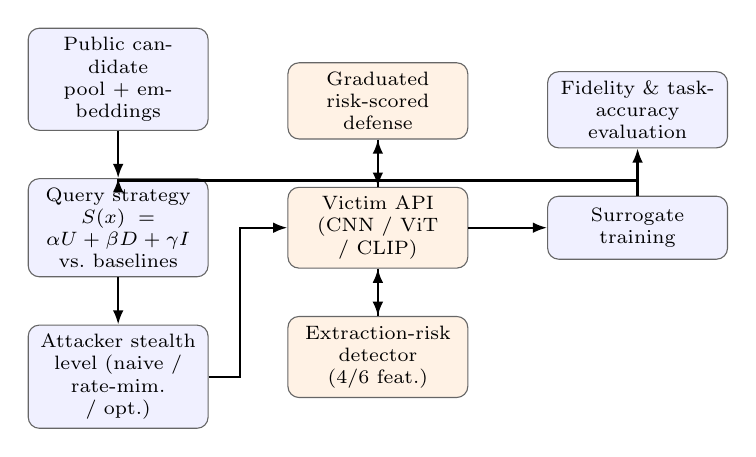
\begin{tikzpicture}[
    node distance=6mm and 8mm,
    box/.style={draw, rounded corners, align=center, minimum height=8mm, font=\scriptsize,
                fill=blue!6, draw=black!60, text width=2.05cm},
    dbox/.style={draw, rounded corners, align=center, minimum height=8mm, font=\scriptsize,
                fill=orange!10, draw=black!60, text width=2.05cm},
    arr/.style={-{Latex[length=1.8mm]}, thick}
]
\node[box] (pool) {Public candidate\\pool + embeddings};
\node[box, below=of pool] (strat) {Query strategy\\$S(x)=\alpha U+\beta D+\gamma I$\\vs.\ baselines};
\node[box, below=of strat] (stealth) {Attacker stealth\\level (naive /\\rate-mim.\ / opt.)};
\node[dbox, right=10mm of strat] (api) {Victim API\\(CNN / ViT / CLIP)};
\node[dbox, above=of api] (defense) {Graduated risk-scored\\defense};
\node[dbox, below=of api] (detector) {Extraction-risk\\detector (4/6 feat.)};
\node[box, right=10mm of api] (surrogate) {Surrogate\\training};
\node[box, above=of surrogate] (eval) {Fidelity \&\ task-\\accuracy evaluation};

\draw[arr] (pool) -- (strat);
\draw[arr] (strat) -- (stealth);
\draw[arr] (stealth.east) -| ++(4mm,0) |- (api.west);
\draw[arr] (api) -- (surrogate);
\draw[arr] (surrogate) -- (eval);
\draw[arr] (surrogate.north) |- ($(strat.east)+(0,6mm)$) -| (strat.north);
\draw[arr] (api) -- (defense);
\draw[arr] (detector) -- (api);
\draw[arr] (api) -- (detector);
\draw[arr] (defense) -- (api);
\end{tikzpicture}
\caption{Extraction pipeline: queries are scored and paced, then sent to the
victim API; a detector and defense monitor the query stream.}
\label{fig:pipeline}
\end{figure}

\subsection{Victim Models}
\label{sec:victims}

We train three victim families, all using a linear-probing regime (frozen backbone plus a trained
classification head, where applicable) so that RQ1/H1 cross-family comparisons are architecture
apples-to-apples: (i) a ResNet-18 convolutional network trained end-to-end as the CNN baseline
(the original design target was ResNet-50; ResNet-18 was substituted for pilot-scale training
time); (ii) a small ViT (a ViT-B/16-scale architecture from the \texttt{timm} library) trained as a
linear probe; and (iii) a CLIP ViT-B/32 image encoder~\cite{radford2021clip} with a frozen backbone
and a trained linear classification head. Each dataset is split into a victim-private training
partition, which the attacker never accesses, and a public candidate pool, from which the attacker
draws query images, following the disjoint-pool requirement standard in the
literature~\cite{orekondy2019knockoff-context}.

\subsection{Simulated Query API}

The victim is wrapped in a simulated MLaaS-style query function that accepts a batch of images and
returns a configurable output type: hard label, top-$k$ ranking, or full confidence vector.
This lets the same attack code be evaluated under different output-knowledge assumptions and lets
the defense stage coarsen the output type as a graduated response (Section~\ref{sec:defense}).

\subsection{Candidate Pool and Embedding Index}

For the diversity term $D(x)$, every candidate image in the public pool is embedded once, offline,
using a surrogate-independent, pretrained ResNet-18 penultimate-layer feature extractor. This
embedding index is architecture-agnostic with respect to the victim and is reused across strategies
and victim families, so its computation is amortised and does not count against the query budget.

\subsection{Baseline Query- Selection Strategies}

We implement four baselines, each selecting a batch of \texttt{batch\_size} candidates per round:
\begin{itemize}
\item \textbf{Random} -- uniform sampling from the unqueried pool.
\item \textbf{Class-balanced} -- sampling that greedily equalises the surrogate's current
predicted-class distribution among queried samples.
\item \textbf{Uncertainty} -- entropy-based active-learning sampling: candidates with highest
surrogate predictive entropy are queried first.
\item \textbf{Diversity} -- a farthest-point / minimum-distance-to-already-queried heuristic in the
pretrained embedding space, so that queries spread out rather than cluster.
\end{itemize}

\subsection{Proposed Adaptive Strategy}
\label{sec:adaptive}

The adaptive strategy scores every unqueried candidate $x$ as
\begin{equation}
S(x) = \alpha\, U(x) + \beta\, D(x) + \gamma\, I(x),
\label{eq:adaptive}
\end{equation}
and queries the top-\texttt{batch\_size} scoring candidates each round, where:
\begin{itemize}
\item $U(x)$ is the surrogate's predictive entropy on $x$ (uncertainty);
\item $D(x)$ is the minimum embedding-space distance from $x$ to any already-queried point
(diversity), computed on the same pretrained embedding index as the diversity baseline; and
\item $I(x)$ is an \emph{information-gain proxy}. Because the victim is black-box, the true
information gain -- the Kullback--Leibler divergence between the surrogate and the (unknown)
victim posterior -- cannot be computed directly. We approximate $I(x)$ by the drop in the
surrogate's confidence margin under a small input perturbation, i.e.\ points whose surrogate
prediction is locally unstable are treated as more informative to query next. We report this
explicitly as a design choice and a defensible but replaceable proxy, following the scope
statement in Section~\ref{sec:discussion}, rather than an oversight.
\end{itemize}
The weights $\alpha,\beta,\gamma$ are tuned by grid search over the simplex
$\{(\alpha,\beta,\gamma): \alpha+\beta+\gamma=1,\ \alpha,\beta,\gamma\ge 0\}$ at a fixed evaluation
budget, with results reported in Section~\ref{sec:results-tuning}.

\subsection{Attack Loop and Surrogate Training}

The generic attack loop is strategy-agnostic: at each round it (i) scores the unqueried candidate
pool under the active strategy, (ii) selects a batch, (iii) queries the victim API, (iv)
incrementally fine-tunes the surrogate on the newly labelled batch for a fixed number of epochs
per round, and (v) repeats until the query budget $B$ is exhausted. \emph{Fidelity} is measured as
the fraction of a held-out evaluation set on which the surrogate's prediction agrees with the
victim's prediction; \emph{task accuracy} is measured against ground-truth labels on the same
evaluation set.

\subsection{Few-Call and Data-Free Baselines}

We additionally reproduce two published baselines that remove the public-candidate-pool assumption.
\textbf{ASPKD}~\cite{hondru2025aspkd} generates a proxy dataset with a diffusion model, actively
queries only a limited, uncertainty-selected subset of it against the victim, pseudo-labels the
remaining proxy images via latent-space nearest-neighbour propagation from the surrogate (at no
extra query cost), and trains with a self-paced curriculum ordered from high- to low-confidence
pseudo-labels. \textbf{Stealix-lite}, a simplified reproduction of the prompt-evolution idea
in~\cite{zhuang2025stealix}, evolves text prompts for a pre-trained diffusion model via a small
genetic-algorithm loop driven by victim feedback, rather than relying on known class names or
hand-crafted prompts, to synthesise query images. We evaluate both under the same query-budget
protocol as the pool-based strategies for direct comparability.

\subsection{Attacker Stealth Levels}
\label{sec:stealth}

We instrument three stealth levels for the query stream, following the three-level taxonomy also
used in the detection literature~\cite{zhou2024inversionguided}:
\begin{itemize}
\item \textbf{Naive} -- queries are issued as fast as possible with no pacing constraint.
\item \textbf{Rate-mimicking} -- inter-query timestamps are generated to match a legitimate
traffic-rate distribution (simulated via timestamp generation rather than real request throttling).
\item \textbf{Stealth-optimized} -- rate-mimicking pacing \emph{plus} a diversity-constrained batch
selection in embedding space, so that queries do not exhibit the near-duplicate/high-coverage
signature that a naive attacker leaves behind.
\end{itemize}

\subsection{Extraction-Risk Detector}

For each session (an attack run, or a simulated legitimate-user session), we extract behavioural
features and train a logistic-regression classifier to label the session as \emph{legitimate} or
\emph{extraction}. We compare two feature sets: a four-feature \textbf{detector v2} (query rate,
near-duplicate rate under an embedding-distance threshold, and class-distribution drift, expanded
to four features) trained on synthetic sessions, and a six-feature \textbf{detector v3} trained on
real attack sessions spanning all three stealth levels above plus simulated legitimate sessions,
adding timing-based features not present in v2.

\subsection{Graduated, Risk-Scored Defense}
\label{sec:defense}

The defense consumes the detector's predicted risk probability (rather than a fixed manual
threshold) and applies a graduated response: normal service $\rightarrow$ confidence coarsening
(bucketed confidence scores) $\rightarrow$ rounded output $\rightarrow$ rate-limiting (fewer
queries served per round) $\rightarrow$ blocking, as risk increases. We sweep three overall
defense-strength settings -- lenient, moderate (default), and strict -- which shift the
risk-to-response mapping, and run the attack loop \emph{live} against each combination of defense
strength and attacker stealth level, rather than replaying a static log, so that the reported
trade-off reflects an adaptive attacker interacting with an adaptive defense.

\section{Experimental Setup}
\label{sec:setup}

\subsection{Datasets and Compute Budget}

Core results use CIFAR-10 (10 classes, $32\times32$ images), split into a victim-private partition
and a disjoint public candidate pool. A generalisation check uses Imagenette, a 10-class subset of
ImageNet-1k (fast.ai mirror), to validate the strongest identified configuration at a larger image
scale without incurring the cost of full ImageNet-1k. All experiments were run on a free-tier
single-GPU budget (NVIDIA T4-class, $\sim$15\,GB, $\sim$30 GPU-hours/week quota), which directly
bounds the scale of the factorial design reported below (Section~\ref{sec:discussion}).

\subsection{Query Budgets and Strategies Compared}

The core strategy comparison uses a query budget of 1{,}000 with grid-tuned adaptive weights
($\alpha=0.4,\beta=0.3,\gamma=0.3$). A separate query-budget sweep evaluates random vs.\ adaptive
at $\{100, 500, 1{,}000, 5{,}000, 10{,}000\}$ queries. Five strategies are compared at the core
budget: random, class-balanced, uncertainty, diversity, and adaptive; the two few-call/data-free
baselines (ASPKD, Stealix-lite) are evaluated separately at matched budgets.

\subsection{Metrics}

We report \emph{fidelity} (surrogate--victim prediction agreement on a held-out evaluation set) as
the primary metric throughout, consistent with the extraction literature's standard
metric~\cite{oliynyk2023survey}. For the core comparison we additionally report five-seed
mean $\pm$ standard deviation, a 95\% confidence interval, a paired $t$-test, and Cohen's $d$. For
the detector we report recall per stealth level and false-positive rate (FPR) on legitimate
sessions; for the defense trade-off we report fidelity-under-defense alongside legitimate-user
accuracy-under-defense, so that any utility cost imposed on legitimate traffic is visible alongside
the attacker's degraded fidelity.

\section{Results}
\label{sec:results}

\subsection{Strategy Comparison at a Fixed Budget}

Fig.~\ref{fig:strategy} reports single-seed fidelity at a 1{,}000-query budget across the five
pool-based strategies against the CNN victim. Random (0.376) and class-balanced (0.365) sampling
achieved the highest single-seed fidelity, followed by the adaptive strategy (0.324); uncertainty
(0.275) and diversity (0.276) alone were weakest. This ordering motivated the multi-seed
re-evaluation below, since single-seed point estimates at this budget are within a range plausibly
attributable to run-to-run variance.

\begin{figure}[t]
\centering

\includegraphics[width=0.92\linewidth]{figures/fig_strategy_comparison.pdf}
\caption{Single-seed fidelity at a 1{,}000-query budget, CNN victim, across the five pool-based
query-selection strategies.}
\label{fig:strategy}
\end{figure}

\subsection{Weight Tuning and Sensitivity}
\label{sec:results-tuning}

Grid search over $(\alpha,\beta,\gamma)$ selected $\alpha=0.4,\beta=0.3,\gamma=0.3$ as the
best-performing configuration among the eight settings tested (Table~\ref{tab:grid}), with a
substantial spread between the best (0.209) and worst (0.124) configuration, indicating that the
adaptive strategy is sensitive to weight choice at this budget and dataset scale.

\begin{table}[t]
\centering
\caption{Adaptive-Weight Grid Search (Query Budget = 1{,}000, Single Seed)}
\label{tab:grid}
\begin{tabular}{@{}lc@{}}
\toprule
$(\alpha,\beta,\gamma)$ & Fidelity \\
\midrule
0.40, 0.30, 0.30 (selected) & 0.2093 \\
0.00, 0.00, 1.00 & 0.2086 \\
0.50, 0.30, 0.20 & 0.2040 \\
0.34, 0.33, 0.33 & 0.2026 \\
0.00, 1.00, 0.00 & 0.1914 \\
0.20, 0.40, 0.40 & 0.1402 \\
1.00, 0.00, 0.00 & 0.1377 \\
0.50, 0.25, 0.25 & 0.1243 \\
\bottomrule
\end{tabular}
\end{table}

\subsection{Component Ablation}

Table~\ref{tab:ablation} and Fig.~\ref{fig:ablation} report a leave-one-term-out ablation of
Eq.~\eqref{eq:adaptive}. Removing the information-gain proxy $I(x)$ produced the largest drop in
fidelity ($-0.0385$), and removing uncertainty $U(x)$ produced a comparable drop ($-0.0344$);
removing diversity $D(x)$ alone \emph{increased} fidelity ($+0.0255$), suggesting that, at this
budget and pool size, the diversity term trades off against, rather than adds to, the other two
terms.

\begin{table}[t]
\centering
\caption{U/D/I Component Ablation (Query Budget = 1{,}000, Single Seed)}
\label{tab:ablation}
\begin{tabular}{@{}lcc@{}}
\toprule
Configuration & Fidelity & $\Delta$ vs.\ full \\
\midrule
Full (U+D+I) & 0.3236 & -- \\
No U (D+I only) & 0.2892 & $+0.0344$ \\
No D (U+I only) & 0.3491 & $-0.0255$ \\
No I (U+D only) & 0.2851 & $+0.0385$ \\
\bottomrule
\end{tabular}
\end{table}

\begin{figure}[t]
\centering

\includegraphics[width=0.92\linewidth]{figures/fig_ablation.pdf}
\caption{Leave-one-term-out ablation of the adaptive strategy $S(x)=\alpha U+\beta D+\gamma I$.}
\label{fig:ablation}
\end{figure}

\subsection{Few-Call and Data-Free Baselines}

At the matched 1{,}000-query budget, ASPKD achieved a fidelity of 0.3921, above both the adaptive
pool-based strategy (0.3236) and random sampling (0.3764) at this single-seed budget, consistent
with ASPKD's design advantage of pseudo-labelling unqueried proxy samples at zero additional query
cost. The simplified Stealix-lite baseline achieved a substantially lower fidelity (0.1594) at the
same nominal budget, which we attribute to the reduced scope of our reproduction relative to the
full genetic prompt-evolution procedure in~\cite{zhuang2025stealix} (Section~\ref{sec:discussion}).

\subsection{Query-Budget Sweep}

Fig.~\ref{fig:budget} shows fidelity for random and adaptive sampling across query budgets from
100 to 10{,}000 against the CNN victim. At the smallest budget (100 queries) random sampling
(0.224) exceeded adaptive (0.130); the two strategies were comparable at 500--1{,}000 queries; and
adaptive modestly exceeded random at the two largest budgets tested (0.4863 vs.\ 0.4638 at
10{,}000 queries). This pattern -- no low-budget adaptive advantage, and only a modest advantage at
the largest budget tested -- is the opposite of hypothesis H2 in the originating research
proposal (that the adaptive strategy's advantage would be \emph{largest} at low budgets); we
discuss this discrepancy in Section~\ref{sec:discussion}.

\begin{figure}[t]
\centering

\includegraphics[width=0.92\linewidth]{figures/fig_budget_sweep.pdf}
\caption{Fidelity vs.\ query budget (log scale), random vs.\ adaptive, CNN victim.}
\label{fig:budget}
\end{figure}

\subsection{Multi-Seed Statistics}

Table~\ref{tab:multiseed} and Fig.~\ref{fig:multiseed} report five-seed statistics for the core
1{,}000-query comparison. Random sampling achieved a higher mean fidelity than the adaptive
strategy (0.3653 vs.\ 0.3286), and this difference was statistically significant under a paired
$t$-test ($t=-3.35$, $p=0.029$, $n=5$ seeds) with a large effect size (Cohen's $d=-1.50$),
\emph{favouring random sampling} over the adaptive strategy at this budget, dataset, and CNN
victim. We report this result as-is rather than selectively emphasising the single-seed or
larger-budget results in which adaptive performs comparably or better, and discuss the
implications in Section~\ref{sec:discussion}.

\begin{table}[t]
\centering
\caption{Five-Seed Core Comparison with 95\% Confidence Intervals}
\label{tab:multiseed}
\begin{tabular}{@{}lccc@{}}
\toprule
Strategy & Mean $\pm$ std & 95\% CI & \\
\midrule
Random & $0.3653 \pm 0.0135$ & [0.3466, 0.3840] & \\
Adaptive (proposed) & $0.3286 \pm 0.0147$ & [0.3082, 0.3490] & \\
\bottomrule
\end{tabular}
\\[2pt]
\footnotesize Paired $t$-test: $t=-3.35$, $p=0.029$; Cohen's $d=-1.50$ ($n=5$ seeds).
\end{table}

\begin{figure}[t]
\centering

\includegraphics[width=0.92\linewidth]{figures/fig_multiseed_ci.pdf}
\caption{Five-seed mean fidelity with 95\% confidence intervals, random vs.\ adaptive.}
\label{fig:multiseed}
\end{figure}

\subsection{Victim-Family Vulnerability (RQ1/H1)}

Fig.~\ref{fig:family} compares fidelity of the adaptive strategy at a 1{,}000-query budget across
the three victim families. The CLIP ViT-B/32 linear-probe victim was the most vulnerable
(0.4861), followed by the CNN (0.3236); the small ViT victim was the most resistant (0.1464).
Because these are single-seed, single-architecture-instance results per family, we treat this
ordering as a pilot-scale signal that CLIP-style linear probes may be disproportionately easy to
extract via their linearly-separable embedding structure, consistent with the encoder-extraction
literature reviewed in Section~\ref{sec:related}~\cite{liu2022stolenencoder,sha2023contsteal},
rather than a confirmed general claim about ViT vs.\ CLIP robustness, which would require
multi-seed and multi-instance replication.

\begin{figure}[t]
\centering

\includegraphics[width=0.92\linewidth]{figures/fig_victim_family.pdf}
\caption{Adaptive-strategy fidelity at 1{,}000 queries, by victim family (RQ1/H1).}
\label{fig:family}
\end{figure}

\subsection{Imagenette Scale-Up}

At the ImageNet-derived (Imagenette) scale, the adaptive strategy substantially out-performed
random sampling (0.7373 vs.\ 0.3850, single seed, strongest identified CIFAR-10 configuration
re-run at this larger image scale), the largest adaptive advantage observed across any setting in
this study. This is consistent with the interpretation that the adaptive strategy's benefit
increases with input dimensionality and/or dataset complexity, an axis not varied within the
CIFAR-10 experiments above.

\subsection{Extraction-Risk Detector}

Table~\ref{tab:detector} and Fig.~\ref{fig:detector} compare the four-feature (v2) and
six-feature (v3) detectors across the three attacker stealth levels. Both detectors achieved
perfect recall (1.00) against the naive attacker and zero recall against the rate-mimicking
attacker. Against the stealth-optimized attacker, the six-feature detector achieved substantially
higher recall than the four-feature detector (0.56 vs.\ 0.00 per-level; 0.44 vs.\ 0.22 aggregate
recall across all three levels), both at zero false-positive rate (FPR) on the legitimate sessions
tested.

\begin{table}[t]
\centering
\caption{Extraction-Risk Detector Recall by Stealth Level (FPR = 0.00 for Both Detectors)}
\label{tab:detector}
\begin{tabular}{@{}lcc@{}}
\toprule
Stealth level & Detector v2 (4 feat.) & Detector v3 (6 feat.) \\
\midrule
Naive & 1.00 & 1.00 \\
Rate-mimicking & 0.00 & 0.00 \\
Stealth-optimized & 0.00 & 0.56 \\
\midrule
Aggregate recall & 0.222 & 0.444 \\
\bottomrule
\end{tabular}
\end{table}

\begin{figure}[t]
\centering

\includegraphics[width=0.92\linewidth]{figures/fig_detector_recall.pdf}
\caption{Detector recall per attacker stealth level, four-feature (v2) vs.\ six-feature (v3).}
\label{fig:detector}
\end{figure}

\subsection{Security--Utility Trade-Off}

Fig.~\ref{fig:tradeoff} traces fidelity-under-defense across the three defense-strength settings
(lenient, moderate/default, strict) and the three attacker stealth levels; legitimate-user accuracy
under defense was stable at 0.37 across every cell tested, indicating that, on the sessions
simulated, the graduated defense did not measurably degrade service for legitimate traffic while
still reducing attacker fidelity. The strict setting achieved the lowest fidelity against the
rate-mimicking attacker (0.029) but was \emph{not} monotonically the best setting against the
naive attacker (0.240 under strict vs.\ 0.104 under moderate), which we attribute to interaction
effects between the risk-scoring threshold and the specific pacing signature of each stealth level
at this pilot scale, and flag as a configuration meriting a wider strength sweep in future work.

\begin{figure}[t]
\centering

\includegraphics[width=0.92\linewidth]{figures/fig_tradeoff_curve.pdf}
\caption{Fidelity-under-defense across three defense-strength settings and three attacker stealth
levels; legitimate-user accuracy was flat at 0.37 in every cell (not plotted).}
\label{fig:tradeoff}
\end{figure}

\section{Discussion, Limitations, and Threats to Validity}
\label{sec:discussion}

\textbf{Scale.} All core results are obtained on CIFAR-10 with a CNN/ResNet-18 surrogate; the
ImageNet-derived generalisation check uses Imagenette (10 classes), not full ImageNet-1k, and no
ViT-B/16 or CLIP ViT-B/16 run at the originally proposed scale was performed, due to free-tier
GPU memory and time limits. The ViT and CLIP victim-family results (Section~\ref{sec:results},
RQ1/H1) are single-seed and should be read as a pilot-scale signal rather than a confirmed claim.

\textbf{Statistical power.} The multi-seed result in Table~\ref{tab:multiseed} uses $n=5$ seeds,
sufficient for a paired $t$-test and a 95\% confidence interval, but the underlying effect-size
estimate at $n=5$ is itself noisy; we report the confidence-interval width alongside the point
estimate for this reason, and we note that this multi-seed result runs \emph{counter} to the
originating hypothesis (that adaptive sampling would out-perform random), a result we report
un-adjusted rather than only reporting the single-seed or large-budget settings in which the
adaptive strategy performs comparably or favourably. A plausible partial explanation is that the
information-gain proxy $I(x)$ (Section~\ref{sec:adaptive}) is itself noisy at low query counts,
since it depends on a surrogate that is still early in training; the budget-sweep result
(Section~\ref{sec:results}, Fig.~\ref{fig:budget}) is consistent with this, showing the adaptive
strategy's disadvantage shrinking as budget grows.

\textbf{Detector training data.} The extraction-risk detector (Table~\ref{tab:detector}) is trained
on simulated attacker sessions generated by this paper's own strategies, compared against
simulated legitimate sessions, not on real third-party API traffic. Its recall/FPR figures
characterise detectability of \emph{this} attack family under \emph{this} simulation, and should
not be read as a general claim about production API-abuse detection.

\textbf{Information-gain proxy.} As stated in Section~\ref{sec:adaptive}, $I(x)$ is an
explicitly-flagged perturbation-sensitivity proxy for the (intractable, black-box) true information
gain, not an attempt at an exact estimate; the ablation in Table~\ref{tab:ablation} indicates it
contributes the single largest marginal effect among the three terms in Eq.~\eqref{eq:adaptive} at
this budget, but a different, tighter proxy could plausibly change the low-budget result in
Section~\ref{sec:results}.

\textbf{Reproduction fidelity of baselines.} Our Stealix-lite baseline is an explicitly simplified
reproduction of the genetic prompt-evolution procedure in~\cite{zhuang2025stealix} and should not
be read as reproducing the fidelity levels reported in the original paper; the gap we observe
between Stealix-lite and ASPKD (Section~\ref{sec:results}) is at least partially attributable to
this reduced scope rather than solely to a difference between the two underlying methods.

\textbf{What would close these gaps.} A full victim$\times$surrogate architecture matrix at the
originally proposed scale (ResNet-50, full ViT-B/16, full CLIP ViT-B/16), evaluated on full
ImageNet-1k with 3--5 seeds per cell, together with detector evaluation on non-simulated traffic if
such data becomes available, would directly address the three limitations above and is the natural
next phase of this line of work, consistent with the staged-design principle recommended for
compute-constrained systems-security studies~\cite{oliynyk2023survey}.

\section{Conclusion}
\label{sec:conclusion}

We presented a pilot-scale, five-seed empirical study of an adaptive query-selection strategy for
black-box model extraction of vision foundation models, benchmarked against four pool-based
baselines and two published few-call/data-free baselines across CNN, ViT, and CLIP victim
families, and coupled to a three-level attacker stealth model and a graduated, risk-scored
behavioural defense. Contrary to our initial hypothesis, the adaptive strategy did not
significantly out-perform random sampling at the core 1{,}000-query CIFAR-10 budget under
multi-seed statistics, though it showed a substantially larger advantage at the ImageNet-derived
scale, and CLIP-style victims were consistently the most vulnerable of the three families tested.
A six-feature behavioural detector nearly doubled recall against a stealth-optimized attacker
relative to a four-feature baseline at zero false-positive rate, and a graduated defense reduced
attacker fidelity without measurably degrading simulated legitimate-user accuracy. We report these
results with explicit scope limitations (Section~\ref{sec:discussion}) and position the full
victim$\times$surrogate factorial matrix at proposal-target scale, on full ImageNet-1k with
multi-seed statistics throughout, as the direct next phase of this work.

\section*{Reproducibility and Data/Code Availability}
\label{sec:repro}
Consistent with the T-IFS editorial board's guidance on reproducibility for papers presenting
deep-learning techniques, we summarise here the information needed to reproduce every reported
number. All experiments use two publicly available datasets (CIFAR-10; Imagenette, a 10-class
subset of ImageNet-1k distributed by fast.ai) and three publicly available pretrained backbones
(\texttt{torchvision}'s ImageNet-pretrained ResNet-18; \texttt{timm}'s \texttt{vit\_small\allowbreak
\_patch16\_224}; OpenAI's CLIP ViT-B/32 via \texttt{open\_clip}), with no proprietary or
access-restricted data. The victim/surrogate training and query-selection code, the exact
random seeds used for the five-seed statistics in Table~\ref{tab:multiseed}, and the raw logged
fidelity/accuracy values underlying every figure and table in this paper are available at
\url{https://anonymous.4open.science/r/model-extraction-vfm-CE13/}. All reported results were
produced on free-tier single-GPU cloud compute (Section~\ref{sec:setup}); no specialised or
restricted-access hardware was used, so the full pipeline is reproducible on equivalent
consumer-grade or free-tier hardware within the GPU-hour budgets stated in
Section~\ref{sec:discussion}.

\section*{Acknowledgment}
The authors thank the maintainers of the open-source libraries (\texttt{timm}, \texttt{open\_clip},
PyTorch) used in the underlying experiments, and the providers of free-tier GPU compute that made
this pilot-scale study possible.

\bibliographystyle{IEEEtran}
\bibliography{references}

\begin{IEEEbiography}[{\includegraphics[width=0.9in,clip,keepaspectratio]{siraj.png}}]{Raja Siraj Gul}
received the BS degree in Computer Science from Pak-Austria Fachhochschule: Institute of Applied Sciences and Technology Haripur, Pakistan. His research interests include Machine Learning, Deep Learning, Computer Vision, AI Ethics and Safety, trustworthy AI and AI for healthcare with a particular focus on precision medicine and intelligent decision support systems. His work aims to contribute to the development of reliable, ethical and human centered artificial intelligence technologies.
\end{IEEEbiography}

\begin{IEEEbiography}[{\includegraphics[width=0.9in,clip,keepaspectratio]{zaigham.jpeg}}]{Sir Zaigham Abdullah bin Qasim}
is an undergraduate researcher with the School of Computing Sciences at Pak-Austria Fachhochschule Institute of Applied Sciences and Technology, Haripur, Pakistan. His research interests include machine learning, data-driven anomaly detection, and the application of artificial intelligence to health and infrastructure domains.
\end{IEEEbiography}

\begin{IEEEbiography}[{\includegraphics[width=0.9in,clip,keepaspectratio]{anonf.jpeg}}]{Zohha Bint E Sajjad}
is currently pursuing the B.S. degree in Artificial Intelligence from the Department of Information Technology, University of Haripur, Haripur, Pakistan, where she is presently in her seventh semester. Her research interests include Machine Learning, Deep Learning, Computer Vision, and Artificial Neural Networks, with a particular focus on the security and robustness of vision-based AI systems. Her work aims to contribute to the development of reliable and trustworthy machine learning technologies.
\end{IEEEbiography}

\begin{IEEEbiography}[{\includegraphics[width=0.9in,clip,keepaspectratio]{anon.jpeg}}]{Kolawole John Adebayo}
received the B.S. degree in electrical and computer engineering from the COMSATS Institute of Information Technology (CIIT), Abbottabad, Pakistan, in 2013, and the M.S. and Ph.D. degrees in electrical and computer engineering from Sungkyunkwan University, Suwon, South Korea, in 2020. Since 2021, he has been an Assistant Professor with the SinoPak Center for Artificial Intelligence (SPCAI), Pak-Austria Fachhochschule: Institute of Applied Sciences and Technology (PAF-IAST), Haripur, Pakistan. His research interests include medium access control, resource allocation, the Internet of Things, applied artificial intelligence, WLAN, sensor networks, energy harvesting networks, backscatter communication networks, power saving, distributed communication networks, and next-generation communication networks. He is an Associate Member and the Team Lead of European Organization for Nuclear Research (CERN) PAF-IAST Team. He was a recipient of the fully-funded ICT research and development scholarship for undergraduates by the Ministry of Information Technology (IT), Pakistan, and the HEC scholarship under the Human Resource Development (HRD) initiative M.S. leading to the Ph.D. program of faculty development for UESTPS, Phase-1 Batch-IV.
\end{IEEEbiography}

\end{document}
